\section{Natural numbers as grammar}
Math in early history (early childhood) is counting.  Count 
pebbles or beads and give the patterns names
\begin{center}
    $0\defeq$ \underline{\hspace{5mm}}, 
    $1\defeq$ \StrokeOne,
    $2\defeq$ \StrokeTwo,
    $3\defeq$ \StrokeThree,
    $4\defeq$ \StrokeFour,
    $5\defeq$ \StrokeFive,...
\end{center}
One hypothesis for the symbol
``0'' is that it looks like the shape left by removing the last pebble from
a sand table leaving behind no pebbles.

It struck Giuseppe Peano in the early 1900's that tallies would be easier to get
right mathematically than digits. With the following two rules Peano introduced
the natural numbers to the formalism of math.
\begin{quote}
    \textit{
    $N_0$ vale ``numero'', et es nomen commune de 0,1,2, etc.\\
    $0$ $\to$  ``zero''\\
    $+$ $\to$ ``plus''.  Si $a$ es numero, $a+$ indica ``numero sequente $a$''.
    }
\end{quote}
% It is fitting that the Italian is in italics.
(See G. Peano \emph{Formulaire de mathematiques.~I-V}, p.27.)
Replacing $+$ with \StrokeOne ~(and equating \StrokeFive$\defeq$\StrokeFour~\StrokeOne),
Peano's model of numbers is simply the grammar of tallies.

Today notation has evolved.  These numbers are now almost always designated as
\emph{natural numbers} and denoted $\mathbb{N}$.  Instead of $a+$ we now often
write $S~k$  or $S(k)$ calling it the ``successor'' to the natural number $k$.  
Programming however has held closer to the original with notation like 
\code{i++} and \code{++i}.

We mentioned Peano was merely recording a grammar.  Today we write grammars with
list of rules, called \emph{production rules}.  Some rules are to specify what
makes up the alphabet of symbols in our grammar.  For Peano, $0$ and $S$ are the
complete alphabet.  So we may write either $0$ on its own, or we may pre-pend
the symbol $S$ to any existing natural number.  Each rule is given a name called
a \emph{token} (or \emph{tag}) and denoted \code{<Name>}. Since the Walrus
$\defeq$ is our assignment of variables (more on this later), we use the
``astonished Walrus'' $::=$ as assignment of production rules.   Taken together
the grammar is the following, shown next to the childhood grammar for tallies.
\begin{center}
\begin{minipage}{0.4\textwidth}
\begin{gcode}[]
<Nat> ::= 0 
<Nat> ::= S <Nat>
\end{gcode}
\end{minipage}
\hfill
\begin{minipage}{0.45\textwidth}
\begin{gcode}[]
<Tally> ::=  
<Tally> ::= | <Tally>
\end{gcode}
\end{minipage}
\end{center}
In the first rule we are told \code{0} is a natural number, denoted
\code{0:Nat}, just as any whitespace can start a tally. We say that the Natural
number grammar \emph{accepts} \code{0} because it matched some production rule,
and the Tally grammar accepts whitespace, usually denoted $\epsilon$.  In the
second rule if we encounter an \code{S} it must be followed by an \emph{already
known} natural number.  So \code{S0:Nat} but \code{0S} would not be accepted as
it is not found as a production rule.  Graphically we can render accepted words
as paths in directed graph called the \emph{word graph} (not to be confused with
parse trees which would occur at each vertex).
\begin{center}
    \begin{tikzpicture}
        \node (0) at (0,0) {0};
        \node (1) at (3,0) {S0};
        \node (2) at (6,0) {SS0};
        \draw[thick,->] (0) edge["S"] (1);
        \draw[thick,->] (1) edge["S"] (2);
    \end{tikzpicture}
\end{center}
The power of the ``already known'' clause of the rules is to prevent ambiguity 
with terms like $n=$\code{SSS....} where the \code{S} continue forever.
See if we remove on \code{S} form $n$, the string is the same as $n$.
Since we are engaged in deciding if $n$ is a natural number and its substring 
is $n$, it is not of the form \code{S k} for \code{k:Nat}.  Hence the grammar 
rejects such an $n$.  Grammar's like these are called \emph{primitive recursive}
meaning that the recursion can only depend backwards 
in history.

% \begin{remark}
%     Some argue that $0$ does not belong in $\mathbb{N}$ because 
%     we begin counting at $1$.  Others argue that Peano's postulates
%     clarify that $0$ is a natural number, and even if you decide to write 
%     it as 1 or 42 it will behave in every way like $0$, in that adding 
%     will by the first term will change nothing.
% \end{remark}

\begin{definition}
    The words (also called strings) of letters accepted by a grammar is called the grammar's \emph{language}.
\end{definition}

What is important is to notice also what is not in a language.  We 
say the grammar \emph{rejects} such strings.  In the Natural 
number's grammar \code{0S} is rejected as there is no production 
rule to match it.

\begin{remark}
    In natural languages, the building blocks of grammar 
    comprised of words (or at least phonemes), as would be found in a dictionary.  The grammar clarifies what it means to accept a string of 
    words as a sentence. The vocabulary used above reflects more the 
    tradition of languages like Chinese where entire words can be characters 
    in the alphabet and strings of characters are sentences.
\end{remark}

\begin{definition}
A production rule that appears more than once is called \emph{inductive}.
An accepted short hand for inductive productions rules is to name it once 
and separate the cases by $\mid$, for instance,
\code{<Nat>::= 0 | S <Nat>} or 
\begin{center}
\begin{gcode}[]
<Nat> ::= 0 
        | S <Nat>
\end{gcode}
\end{center}
\end{definition}


Because of this notation for inductive types we will limit our use of tallies
to avoid confusion.

    
\subsection{Grammar is inflexible}

One might argue that Peano's numbers are different to the tally we all use.  For example, in a tally we might 
add strokes to either side.  For instance:
\begin{center}
    \StrokeOne~\StrokeTwo = \StrokeThree = \StrokeTwo~\StrokeOne,
    i.e.\ $1+2=3=2+1$.
\end{center}
This is possible but requires a different grammar.  To make the point clear let us 
use $L$ for tallies on the left and $R$ for tallies on the right, and use a $0$ for 
the empty space.
\begin{center}
\begin{gcode}[]
<LRNat> ::= 0
         | L <LRNat>
         | <LRNat> R
\end{gcode}
\end{center}
If we graph some of the accepted words we see an immediate difference.
Note here we include parentheses to clarify the order in which 
words like \code{L0R} can be accepted.  Those are not part of the 
original string but indicate how the grammar sees these.
\begin{center}
    \begin{tikzpicture}[xscale=1.3]
        \node[draw] (LL0) at (-4,-2) {
            \begin{tikzpicture}[scale=0.5]
                \node[scale=0.5] (0) at (0,0) {0};
                \node[scale=0.5] (L0) at (-1,-1) {L0};
                \node[scale=0.5] (LL0) at (-2,-2) {LL0};
                \draw[-] (0) -- (L0) -- (LL0);
            \end{tikzpicture}};
        \node[draw] (RL0) at (0,2) {
            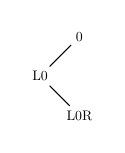
\begin{tikzpicture}[scale=0.5]
                \node[scale=0.5] (0) at (0,0) {0};
                \node[scale=0.5] (L0) at (-1,-1) {L0};
                \node[scale=0.5] (RL0) at (0,-2) {L0R};
                \draw[-] (0) -- (L0) -- (RL0);
            \end{tikzpicture}};

        \node[draw] (L0) at (-2, 0) {
            \begin{tikzpicture}[scale=0.5]
                \node[scale=0.5] (0) at (0,0) {0};
                \node[scale=0.5] (L0) at (-1,-1) {L0};
                \draw[-] (0) -- (L0);
            \end{tikzpicture}};
        \node[draw] (0) at (0,0) {0};
        \node[draw] (0Rx) at ( 2, 0) {
            \begin{tikzpicture}[scale=0.5]
                \node[scale=0.5] (0) at (0,0) {0};
                \node[scale=0.5] (0R) at ( 1,-1) {0R};
                \draw[-] (0) -- (0R);
            \end{tikzpicture}};

        \node[draw] (0RR) at ( 4, 2) {
            \begin{tikzpicture}[scale=0.5]
                \node[scale=0.5] (0) at (0,0) {0};
                \node[scale=0.5] (0R) at (1,-1) {0R};
                \node[scale=0.5] (0RR) at ( 2,-2) {0RR};
                \draw[-] (0) -- (0R) -- (0RR);
            \end{tikzpicture}};
        \node[draw] (0RL) at (0,-2) {
            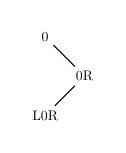
\begin{tikzpicture}[scale=0.5]
                \node[scale=0.5] (0) at (0,0) {0};
                \node[scale=0.5] (0R) at ( 1,-1) {0R};
                \node[scale=0.5] (0RL) at (0,-2) {L0R};
                \draw[-] (0) -- (0R) -- (0RL);
            \end{tikzpicture}};

        \draw[thick,->] (L0) edge["L"] (LL0);
        \draw[thick,->] (L0) edge["R"] (RL0);
        
        \draw[thick,->] (0) edge["L"] (L0);
        \draw[thick,->] (0) edge["R"] (0Rx);

        \draw[thick,->] (0Rx) edge["R"] (0RR);
        \draw[thick,->] (0Rx) edge["L"] (0RL);
    \end{tikzpicture}
\end{center}
% \begin{center}
%     \code{L0:LRNat}, \code{0R:LRNat}, and \code{L0R:LRNat}.
% \end{center}
Yet nothing in this treats \code{L0}=\code{0R}.  So left/right 
tallies are in the sense of the grammar quite different.  If we 
want to overcome this we will need to add more properties to the 
semantics (meaning) of grammar such as by adding ways rewrite.
This will come up when we later discuss relations.

This grammar is also ambiguous in that $L0R$ can be accepted by more than one
production rule.  This hints further lingering problems to solve.
some further

\subsection{Realizing grammar}

We do well to acknowledge inductive types of data as basic programs. Computers
understand this much. Listing~\ref{lst:peano} shows two programs you could run
today that implement Peano's idea. There are of course many differences.
Visibly, the left-hand side favors mathematically minded symbolic notation and
economizes even on parentheses in the spirit of ``$\sin x$'' notation. Meanwhile
the right-hand side favors a verbose imitation of natural language and prefers
the $\sin(x)$ notation.  Set the differences aside.

\begin{lstfloat}
\begin{center}
\begin{minipage}{0.34\textwidth}
\begin{Fcode}[]
data Nat = Z 
         | S k

zero = Z
two = S (S zero)
\end{Fcode}
\end{minipage}
\hfill
\begin{minipage}{0.65\textwidth}
\begin{Pcode}[language=Sava]
class Nat
    case Zero() extends Nat
    case Next(k:Nat) extends Nat
sealed  // no more cases
zero = new Zero()
two = new Next(new Next(zero))
\end{Pcode}
\end{minipage}
\end{center}
\caption{Peano's natural numbers programmed in two different languages.}
\label{lst:peano}
\end{lstfloat}
    

Even without a deep understanding of these programs, one can make out the
contours of Paeno's definitions.  Both use a mix of keywords (in blue) to tell
our system to prepare a new type (or class) of data that will be called
\code{Nat}.  Then they instruct the system to accept exactly two ways to make
such data. It may be some initial state, \code{Z}, respectively \code{Zero},
that depends on nothing; otherwise, we must give data \code{k} of type
\code{Nat}, denoted \code{k:Nat}, which will then produce new data \code{S k},
respectively \code{Next(k)}.  In many systems the keyword \code{new} is 
used to help clue the reader into the fact that this is some data being now 
created.  It helps remind us that numbers do not  exists on their own, 
we have to expend resources (energy \& storage) to create them. 

